\chapter{Módulos no implementados}
\label{app:cu_no_implementados}

A continuación se presentan los módulos que no serán implementados en éste primer prototipo del SNS deportivo.

\section{Módulo de administración de entrenadores}

\begin{figure}[!htb]
  \begin{center}
    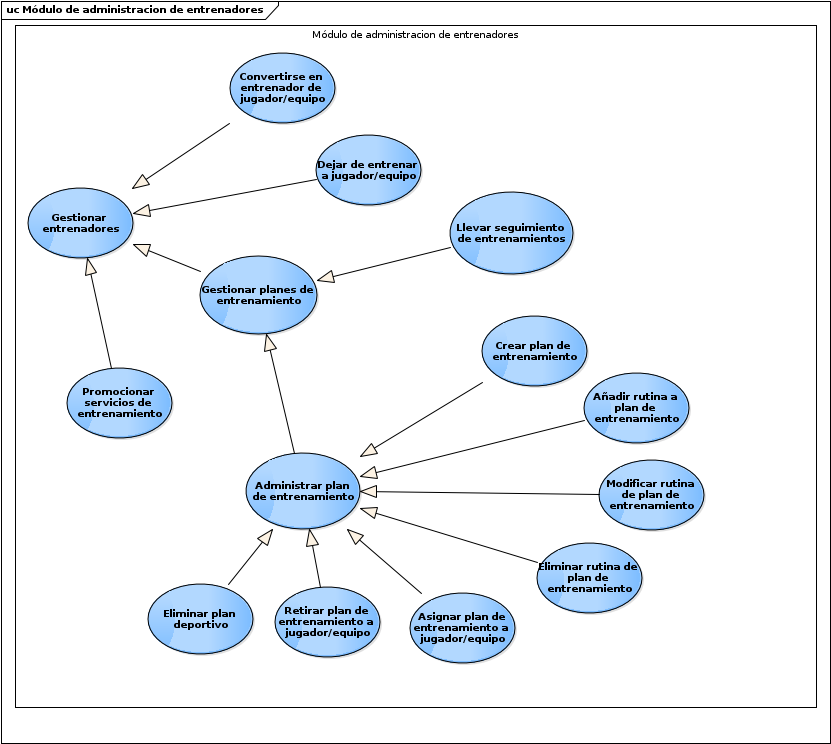
\includegraphics[width=11cm]{./imagenes/casos_uso/gestion_entrenador.png}
    \caption{Módulo de administración de entrenadores}
    \label{fig:cu_admin_ent}
    \textbf{Fuente:} Autores\textbf{Fuente:} Autores \\
    \textbf{Ver anexo en:} /Proyecto/imagenes/casos\_uso/gestion\_entrenador.png
  \end{center}
\end{figure}

Sobre éste módulo de entrenadores se han recopilado las funcionalidades que pretende ofrecer el SNS deportivo a los entrenadores. Dichas funcionalidades resumen la capacidad de los actores deportivos entrenadores de ofrecer su servicio deportivo a la comunidad deportiva y de hacer el seguimiento de entrenamientos con sus entrenados desde el SNS.

\section{Módulo de administración de torneos}

\begin{figure}[!htb]
  \begin{center}
    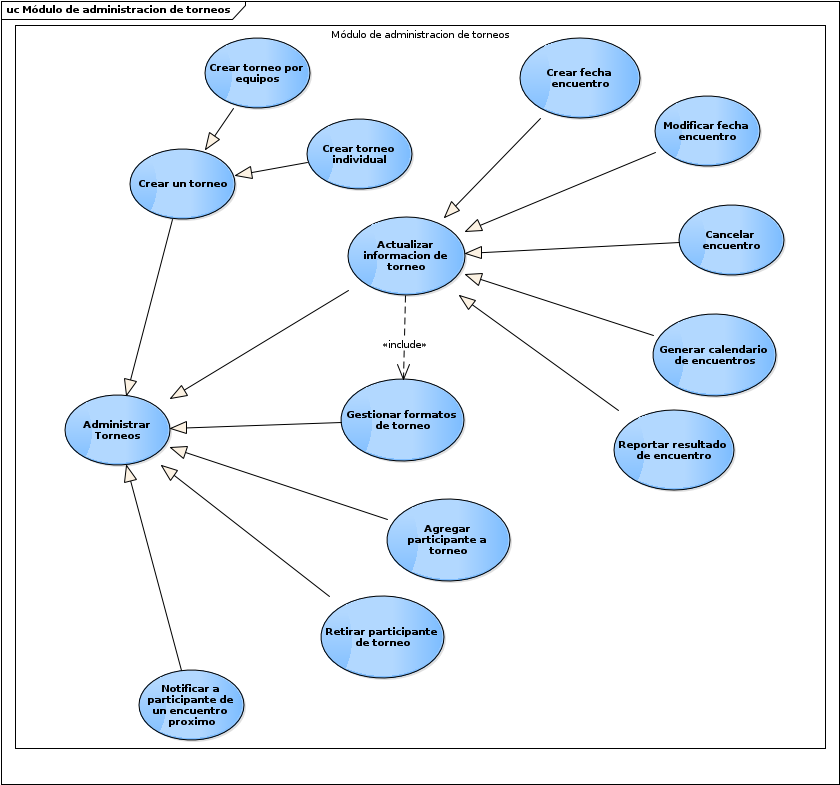
\includegraphics[width=11cm]{./imagenes/casos_uso/gestion_torneo.png}
    \caption{Módulo de administración de torneos}
    \label{fig:cu_admin_torn}
    \textbf{Fuente:} Autores \\
    \textbf{Ver anexo en:} /Proyecto/imagenes/casos\_uso/gestion\_torneo.png
  \end{center}
\end{figure}

El módulo de administración de torneos es una extensión al módulo de administración de eventos debido a que un torneo es también considerado un evento deportivo. Particularmente se dan funcionalidades de administración de información del torneo, así como la adición y retiro de participantes al torneo y, a su vez, la gestión del formato que se le quiera dar al torneo (que tipo de eliminatorias se van a llevar, por ejemplificar).

\section{Módulo de gestión de patrocinios}

\begin{figure}[!htb]
  \begin{center}
    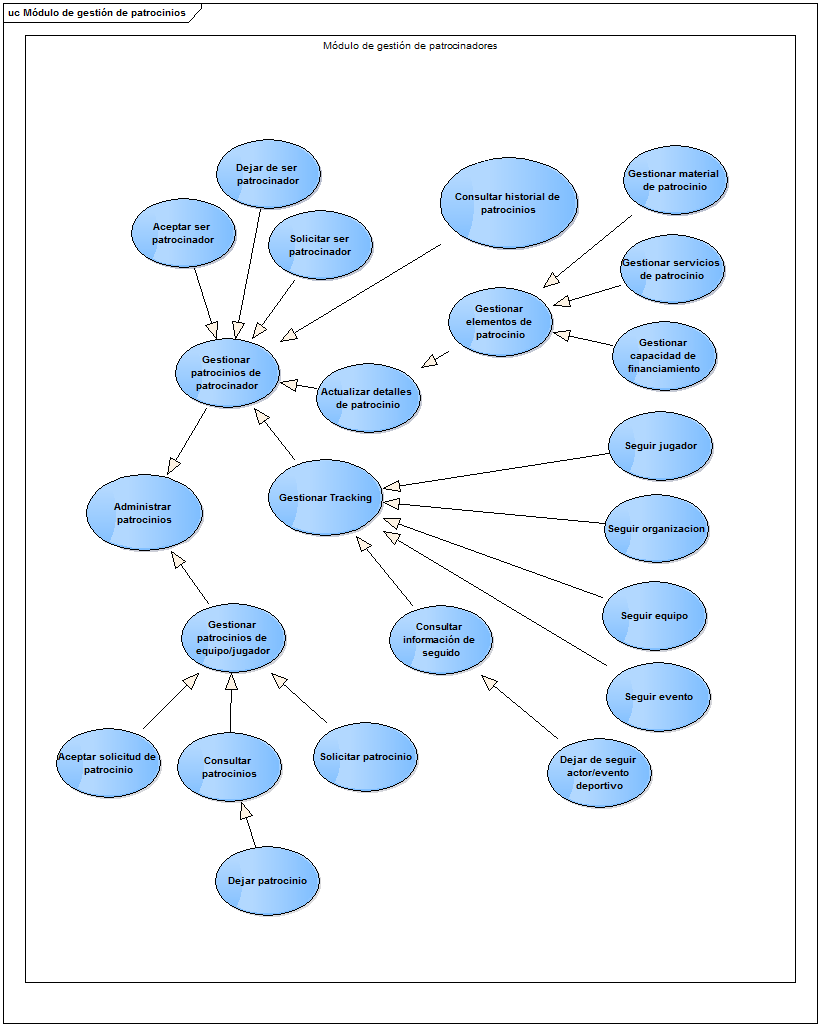
\includegraphics[width=11cm]{./imagenes/casos_uso/gestion_patrocinios.png}
    \caption{Módulo de gestión de patrocinios}
    \label{fig:cu_gest_patr}
    \textbf{Fuente:} Autores \\
    \textbf{Ver anexo en:} /Proyecto/imagenes/casos\_uso/gestion\_patrocinios.png
  \end{center}
\end{figure}

Este módulo ofrece funcionalidades tanto para patrocinador como patrocinado, indicando aquí que sólo el actor correspondiente (siendo patrocinador o patrocinado) puede acceder a uno de las dos grandes funcionalidades que se pueden apreciar: Por parte del patrocinador, se prestan funcionalidades de seguimiento de usuarios candidatos a patrocinar, así como la petición de patrocinio y consulta de patrocinios; Por parte del jugador, se ofrecen funcionalidades similares pero sin poder hacer seguimiento.

\section{Módulo de administración de equipos y grupos deportivos}

\begin{figure}[!htb]
  \begin{center}
    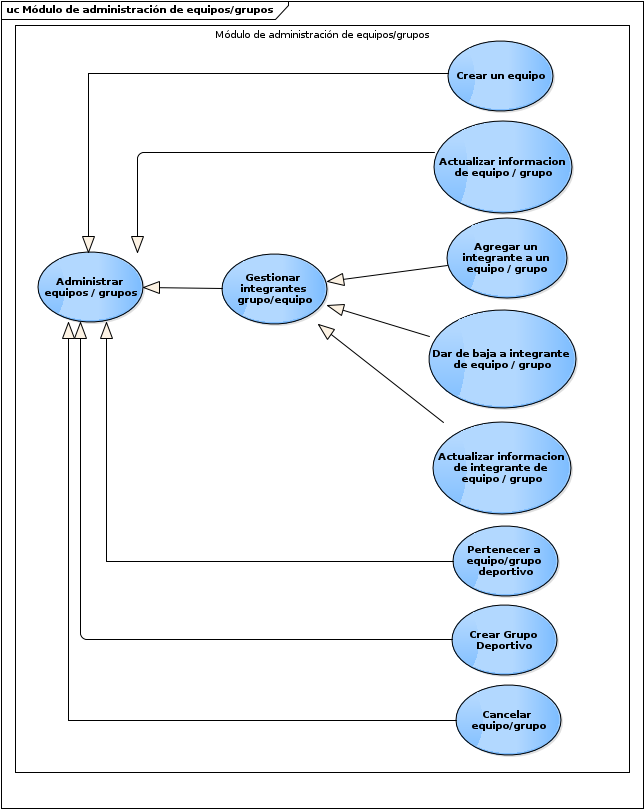
\includegraphics[width=11cm]{./imagenes/casos_uso/gestion_equipo_grupo.png}
    \caption{Módulo de administración de equipos y grupos deportivos}
    \label{fig:cu_admin_equip_grup}
    \textbf{Fuente:} Autores \\
    \textbf{Ver anexo en:} /Proyecto/imagenes/casos\_uso/gestion\_equipo\_grupo.png
  \end{center}
\end{figure}

A éste módulo le corresponde ofrecer funcionalidades de administración de equipos y grupos deportivos. Se decidió dejar la administración de ámbos conceptos (equipo y grupo deportivo) en el mismo módulo ya que, para efectos de las funcionalidades ofrecidas por el SNS, son bastante similares. Adicionalmente, un grupo deportivo no podrá utilizar todas las funcionalidades ofrecidas en el presente módulo, esto debido a su caracter limitado de grupo informal.

\section{Módulo de difusión de información}


\begin{figure}[!htb]
  \begin{center}
    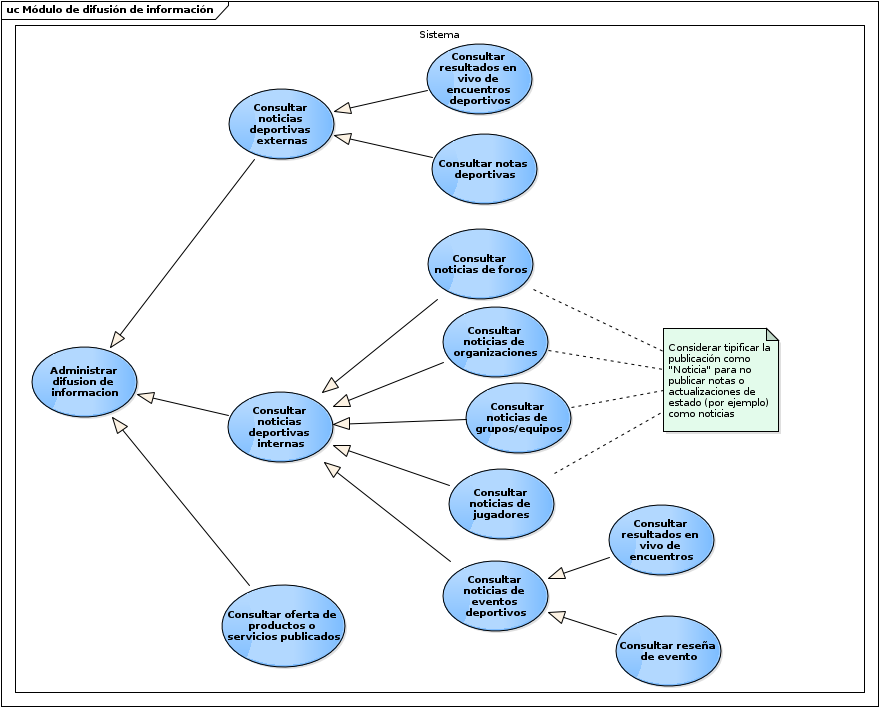
\includegraphics[width=11cm]{./imagenes/casos_uso/difusion_informacion.png}
    \caption{Módulo de administración de equipos y grupos deportivos}
    \label{fig:cu_admin_equip_grup}
    \textbf{Fuente:} Autores \\
    \textbf{Ver anexo en:} /Proyecto/imagenes/casos\_uso/difusion\_informacion.png
  \end{center}
\end{figure}

Este modulo ofrece al usuario la funcionalidad de buscar noticias, ya esan internas (originadas y/o publicadas en la aplicacion) o externas (publicadas por sitios de noticias externas).

\section{Módulo de estadísticas}

\begin{figure}[!htb]
  \begin{center}
    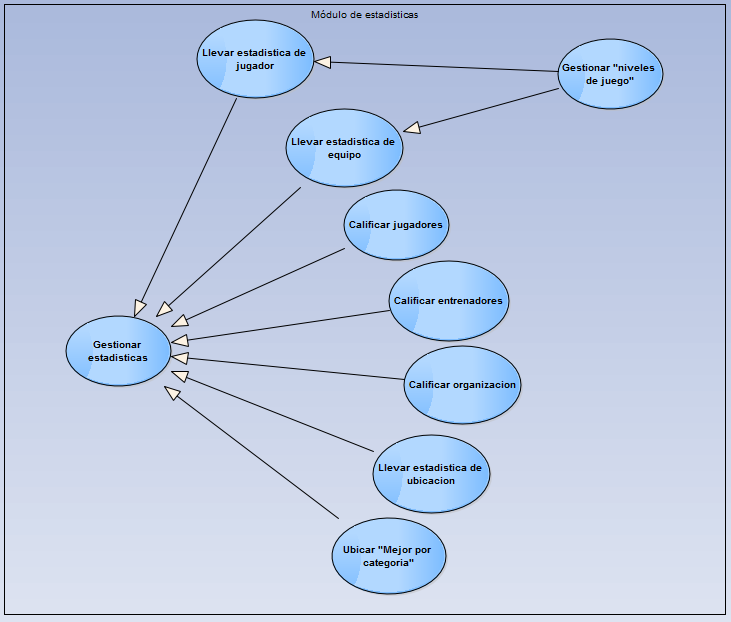
\includegraphics[width=11cm]{./imagenes/casos_uso/gestion_estadisticas.png}
    \caption{Módulo de estadísticas}
    \label{fig:cu_estad}
    \textbf{Fuente:} Autores \\
    \textbf{Ver anexo en:} /Proyecto/imagenes/casos\_uso/gestion\_estadisticas.png
  \end{center}
\end{figure}

Las funcionalidades ofrecidas por éste módulo son proporcionadas por el SNS para dar soporte estadístico a cáda uno de los objetos de negocio especificados en el capítulo \ref{chap:arquitectura}, en lo que se refiere al proceso estadístico. Como adición, visto desde los requerimientos funcionales, se da una funcionalidad de llevar el mejor calificado en cáda uno de los objetos de negocio, con tal de que el usuario del SNS pueda ver aquellos objetos de negocio destacados cuando el lo requiera.

\clearpage

\section{Módulo de gestión de self-expression}

\begin{figure}[!htb]
  \begin{center}
    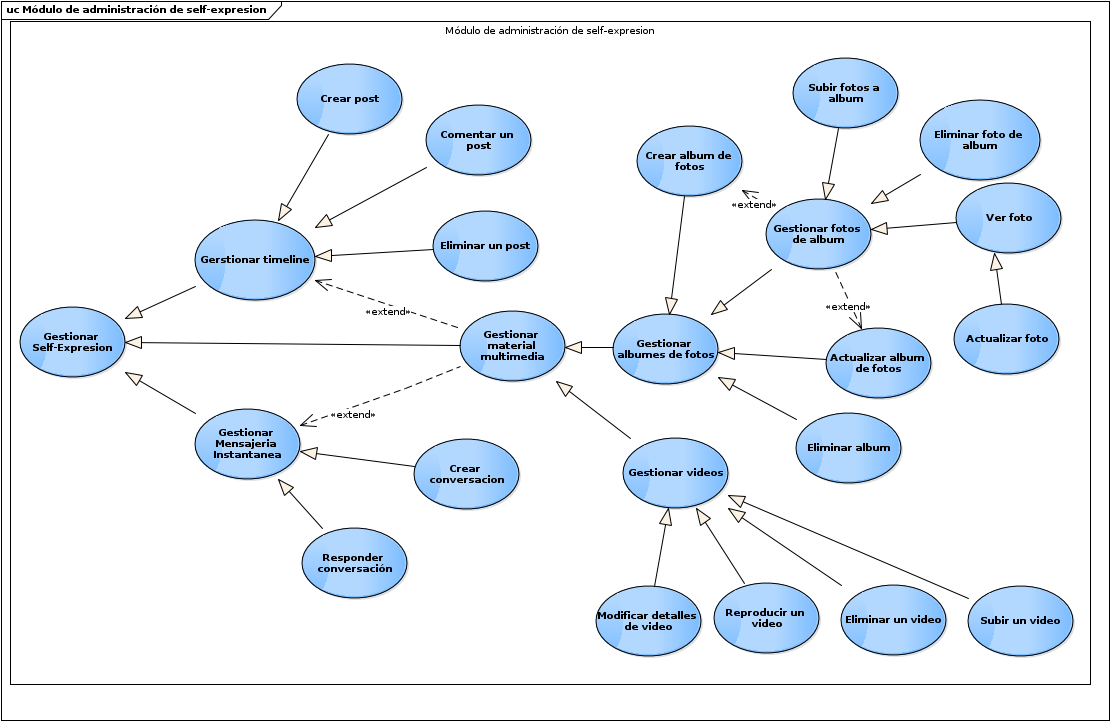
\includegraphics[width=11cm]{./imagenes/casos_uso/gestion_self_sharing.png}
    \caption{Módulo de gestión de self-expression}
    \label{fig:cu_self_shar}
    \textbf{Fuente:} Autores \\
    \textbf{Ver anexo en:} /Proyecto/imagenes/casos\_uso/gestion\_self\_sharing.png
  \end{center}
\end{figure}

Este módulo ofrece funcionalidades propias de redes social similares a Facebook. Por medio de éste el usuario podrá manejar la comunicación de él con sus amigos a traves de un timeline, del servicio de mensajería instantánea y de la posibilidad de compartir elementos multimedia como lo son videos y fotos, así como también mostrar y actualizar su información personal.

\section{Módulo de gestión del conocimiento}

\begin{figure}[!htb]
  \begin{center}
    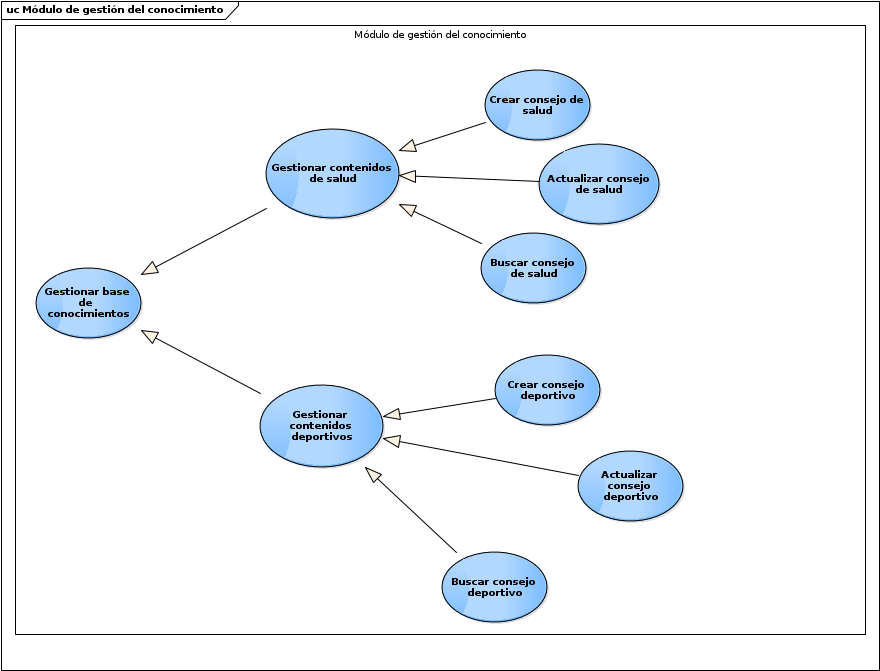
\includegraphics[width=11cm]{./imagenes/casos_uso/gestion_conocimiento.png}
    \caption{Módulo de gestión de self-expression}
    \label{fig:cu_self_shar}
    \textbf{Fuente:} Autores \\
    \textbf{Ver anexo en:} /Proyecto/imagenes/casos\_uso/gestion\_conocimiento.png
  \end{center}
\end{figure}

Este modulo ofrece al usuario la funcionalidad de buscar o publicar información relacionada a los deportes. En el alcance actual se tiene contemplados contenidos deportivos (relacionados a la práctica de un deporte) y de salud (relacionados a consejos y cuidados orientados a los deportistas).